% Options for packages loaded elsewhere
% Options for packages loaded elsewhere
\PassOptionsToPackage{unicode}{hyperref}
\PassOptionsToPackage{hyphens}{url}
\PassOptionsToPackage{dvipsnames,svgnames,x11names}{xcolor}
%
\documentclass[
  10pt,
  letterpaper,
  DIV=11,
  numbers=noendperiod]{scrartcl}
\usepackage{xcolor}
\usepackage[lmargin=0.5in,rmargin=0.5in,tmargin=0.5in,bmargin=0.5in]{geometry}
\usepackage{amsmath,amssymb}
\setcounter{secnumdepth}{-\maxdimen} % remove section numbering
\usepackage{iftex}
\ifPDFTeX
  \usepackage[T1]{fontenc}
  \usepackage[utf8]{inputenc}
  \usepackage{textcomp} % provide euro and other symbols
\else % if luatex or xetex
  \usepackage{unicode-math} % this also loads fontspec
  \defaultfontfeatures{Scale=MatchLowercase}
  \defaultfontfeatures[\rmfamily]{Ligatures=TeX,Scale=1}
\fi
\usepackage{lmodern}
\ifPDFTeX\else
  % xetex/luatex font selection
\fi
% Use upquote if available, for straight quotes in verbatim environments
\IfFileExists{upquote.sty}{\usepackage{upquote}}{}
\IfFileExists{microtype.sty}{% use microtype if available
  \usepackage[]{microtype}
  \UseMicrotypeSet[protrusion]{basicmath} % disable protrusion for tt fonts
}{}
\usepackage{setspace}
% Make \paragraph and \subparagraph free-standing
\makeatletter
\ifx\paragraph\undefined\else
  \let\oldparagraph\paragraph
  \renewcommand{\paragraph}{
    \@ifstar
      \xxxParagraphStar
      \xxxParagraphNoStar
  }
  \newcommand{\xxxParagraphStar}[1]{\oldparagraph*{#1}\mbox{}}
  \newcommand{\xxxParagraphNoStar}[1]{\oldparagraph{#1}\mbox{}}
\fi
\ifx\subparagraph\undefined\else
  \let\oldsubparagraph\subparagraph
  \renewcommand{\subparagraph}{
    \@ifstar
      \xxxSubParagraphStar
      \xxxSubParagraphNoStar
  }
  \newcommand{\xxxSubParagraphStar}[1]{\oldsubparagraph*{#1}\mbox{}}
  \newcommand{\xxxSubParagraphNoStar}[1]{\oldsubparagraph{#1}\mbox{}}
\fi
\makeatother


\usepackage{longtable,booktabs,array}
\usepackage{calc} % for calculating minipage widths
% Correct order of tables after \paragraph or \subparagraph
\usepackage{etoolbox}
\makeatletter
\patchcmd\longtable{\par}{\if@noskipsec\mbox{}\fi\par}{}{}
\makeatother
% Allow footnotes in longtable head/foot
\IfFileExists{footnotehyper.sty}{\usepackage{footnotehyper}}{\usepackage{footnote}}
\makesavenoteenv{longtable}
\usepackage{graphicx}
\makeatletter
\newsavebox\pandoc@box
\newcommand*\pandocbounded[1]{% scales image to fit in text height/width
  \sbox\pandoc@box{#1}%
  \Gscale@div\@tempa{\textheight}{\dimexpr\ht\pandoc@box+\dp\pandoc@box\relax}%
  \Gscale@div\@tempb{\linewidth}{\wd\pandoc@box}%
  \ifdim\@tempb\p@<\@tempa\p@\let\@tempa\@tempb\fi% select the smaller of both
  \ifdim\@tempa\p@<\p@\scalebox{\@tempa}{\usebox\pandoc@box}%
  \else\usebox{\pandoc@box}%
  \fi%
}
% Set default figure placement to htbp
\def\fps@figure{htbp}
\makeatother


% definitions for citeproc citations
\NewDocumentCommand\citeproctext{}{}
\NewDocumentCommand\citeproc{mm}{%
  \begingroup\def\citeproctext{#2}\cite{#1}\endgroup}
\makeatletter
 % allow citations to break across lines
 \let\@cite@ofmt\@firstofone
 % avoid brackets around text for \cite:
 \def\@biblabel#1{}
 \def\@cite#1#2{{#1\if@tempswa , #2\fi}}
\makeatother
\newlength{\cslhangindent}
\setlength{\cslhangindent}{1.5em}
\newlength{\csllabelwidth}
\setlength{\csllabelwidth}{3em}
\newenvironment{CSLReferences}[2] % #1 hanging-indent, #2 entry-spacing
 {\begin{list}{}{%
  \setlength{\itemindent}{0pt}
  \setlength{\leftmargin}{0pt}
  \setlength{\parsep}{0pt}
  % turn on hanging indent if param 1 is 1
  \ifodd #1
   \setlength{\leftmargin}{\cslhangindent}
   \setlength{\itemindent}{-1\cslhangindent}
  \fi
  % set entry spacing
  \setlength{\itemsep}{#2\baselineskip}}}
 {\end{list}}
\usepackage{calc}
\newcommand{\CSLBlock}[1]{\hfill\break\parbox[t]{\linewidth}{\strut\ignorespaces#1\strut}}
\newcommand{\CSLLeftMargin}[1]{\parbox[t]{\csllabelwidth}{\strut#1\strut}}
\newcommand{\CSLRightInline}[1]{\parbox[t]{\linewidth - \csllabelwidth}{\strut#1\strut}}
\newcommand{\CSLIndent}[1]{\hspace{\cslhangindent}#1}



\setlength{\emergencystretch}{3em} % prevent overfull lines

\providecommand{\tightlist}{%
  \setlength{\itemsep}{0pt}\setlength{\parskip}{0pt}}



 


\usepackage[dvipsnames,svgnames,x11names]{xcolor}
\usepackage{eso-pic}

\RedeclareSectionCommand[font=\centering\large]{section}
\RedeclareSectionCommand[
  runin=false,
  afterindent=false,
  font = \normalfont\textbf,
  beforeskip=0pt,
  afterskip=0pt]{subsection}

\setlength{\itemsep}{1pt}
\setlength{\parskip}{0pt}
\setlength{\parsep}{0pt}
\setlength{\labelsep}{0pt}
\setlength{\topsep}{0pt}
\setlength{\parsep}{0pt}
\setlength{\partopsep}{0pt}

\pagenumbering{gobble}
\usepackage{fontspec}
\usepackage{multirow}
\usepackage{multicol}
\usepackage{colortbl}
\usepackage{hhline}
\newlength\Oldarrayrulewidth
\newlength\Oldtabcolsep
\usepackage{longtable}
\usepackage{array}
\usepackage{hyperref}
\usepackage{float}
\usepackage{wrapfig}
\KOMAoption{captions}{tableheading}
\makeatletter
\@ifpackageloaded{caption}{}{\usepackage{caption}}
\AtBeginDocument{%
\ifdefined\contentsname
  \renewcommand*\contentsname{Table of contents}
\else
  \newcommand\contentsname{Table of contents}
\fi
\ifdefined\listfigurename
  \renewcommand*\listfigurename{List of Figures}
\else
  \newcommand\listfigurename{List of Figures}
\fi
\ifdefined\listtablename
  \renewcommand*\listtablename{List of Tables}
\else
  \newcommand\listtablename{List of Tables}
\fi
\ifdefined\figurename
  \renewcommand*\figurename{Figure}
\else
  \newcommand\figurename{Figure}
\fi
\ifdefined\tablename
  \renewcommand*\tablename{Table}
\else
  \newcommand\tablename{Table}
\fi
}
\@ifpackageloaded{float}{}{\usepackage{float}}
\floatstyle{ruled}
\@ifundefined{c@chapter}{\newfloat{codelisting}{h}{lop}}{\newfloat{codelisting}{h}{lop}[chapter]}
\floatname{codelisting}{Listing}
\newcommand*\listoflistings{\listof{codelisting}{List of Listings}}
\makeatother
\makeatletter
\makeatother
\makeatletter
\@ifpackageloaded{caption}{}{\usepackage{caption}}
\@ifpackageloaded{subcaption}{}{\usepackage{subcaption}}
\makeatother
\usepackage{bookmark}
\IfFileExists{xurl.sty}{\usepackage{xurl}}{} % add URL line breaks if available
\urlstyle{same}
\hypersetup{
  pdftitle={U.S. Caribbean Snapshot Ecosystem Status Report},
  colorlinks=true,
  linkcolor={blue},
  filecolor={Maroon},
  citecolor={Blue},
  urlcolor={Blue},
  pdfcreator={LaTeX via pandoc}}


\title{U.S. Caribbean \linebreak Snapshot Ecosystem Status Report}
\author{}
\date{}
\begin{document}
\maketitle


\setstretch{1}
\AddToShipoutPictureBG*{%
  \AtPageLowerLeft{%
    
\includegraphics[width=\paperwidth,height=\paperheight]{bg_pg1.jpg}%
  }%
}

\vspace{-2.5cm}
\section{2025}

This is a short-form update to the full 2025 U.S. Caribbean Ecosystem
Status Report (ESR) {[}1{]} highlighting the recent status of
environmental, ecological, and socioeconomic factors. Indicators were
compiled into two categories: tracking performance toward fishery
management objectives and risks to meeting fishery management
objectives.

\vspace{-0.25cm}

\begin{figure}

\begin{minipage}{0.40\linewidth}
\pandocbounded{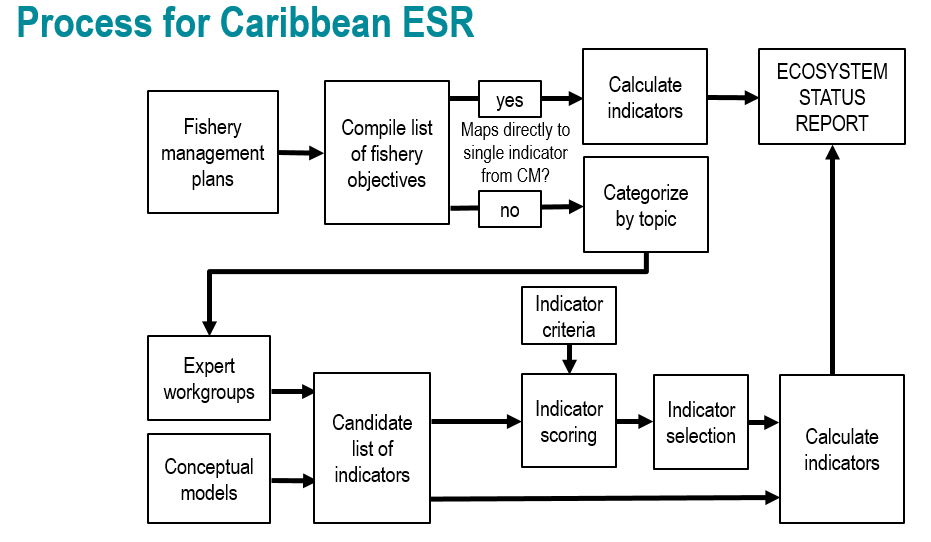
\includegraphics[keepaspectratio]{C:/Users/clger/Documents/My Github Projects/ESR-2pager-template-DRAFT/images/process_flow_chart.png}}
\normalsize\end{minipage}%
%
\begin{minipage}{0.03\linewidth}

\hfill

\end{minipage}%
%
\begin{minipage}{0.57\linewidth}

\section{Overview of recent trends}
\vspace{-0.25cm}

\subsection{Performace indicators}

\begin{itemize}
\tightlist
\item
  17 indicators were compiled to track perfomance towards management
  objectives.
\item
  Indicators were categorized as relating to food production,
  socioeconomic health, equality, engagement and participation, bycatch
  reduction, governance, and protection of ecosystems.
\item
  add some text about indicators
\end{itemize}

\vspace{-0.25cm}
\subsection{Risk indicators}

\begin{itemize}
\tightlist
\item
  13 indicators were compiled to track risks to meeting management
  objectives.
\item
  Indicators track changes in the physical environment and human
  activities.
\item
  Major recent changes in the physical environment include increased sea
  surface temperature, coral bleaching stress, and ocean acidification.
\item
  Other insights?
\end{itemize}

\end{minipage}%

\end{figure}%

\vspace{0.5cm}
\section{Integrated Ecosystem Perspectives}
\vspace{0.05cm}

\subsection{Analysis}

Multivariate methods (principal components analysis and traffic light
plot; see details in full report) were used to synthesize the
information contained in the full suite of indicators.

\subsection{Interpretation}

The traffic plot conveys that many indicator values underwent rapid
change in the period 2017-2021, and the PCA biplots confirm these
patterns as there are larger two-dimensional shifts between these years.
These shifts are most likely driven by several major stressor events in
this time period, including the major hurricanes Maria and Irma (2017)
and the COVID pandemic (2020-2021). Together, the multivariate analyses
suggest that these events have had some destabilizing impacts on the
U.S. Caribbean fishery ecosystem.

\begin{figure}

\begin{minipage}{0.50\linewidth}
\pandocbounded{\includegraphics[keepaspectratio]{../images/traffic.png}}\end{minipage}%
%
\begin{minipage}{0.50\linewidth}
\pandocbounded{\includegraphics[keepaspectratio]{../images/pcas.png}}\end{minipage}%

\end{figure}%

\newpage

\AddToShipoutPictureBG*{%
  \AtPageLowerLeft{%
    
\includegraphics[width=\paperwidth,height=\paperheight]{bg_pg2.jpg}%
  }%
}

\newgeometry{top=0.75in, left=0.75in, right=0.75in, bottom=0.75in}

\global\setlength{\Oldarrayrulewidth}{\arrayrulewidth}

\global\setlength{\Oldtabcolsep}{\tabcolsep}

\setlength{\tabcolsep}{2pt}

\renewcommand*{\arraystretch}{1.5}



\providecommand{\ascline}[3]{\noalign{\global\arrayrulewidth #1}\arrayrulecolor[HTML]{#2}\cline{#3}}

\begin{longtable*}[c]{|p{0.90in}|p{0.75in}|p{2.00in}|p{3.00in}}



\ascline{1.5pt}{666666}{1-4}

\multicolumn{1}{>{\raggedright}m{\dimexpr 0.9in+0\tabcolsep}}{\textcolor[HTML]{000000}{\fontsize{11}{11}\selectfont{\global\setmainfont{Times New Roman}{Indicator}}}} & \multicolumn{1}{>{\raggedleft}m{\dimexpr 0.75in+0\tabcolsep}}{\textcolor[HTML]{000000}{\fontsize{11}{11}\selectfont{\global\setmainfont{Times New Roman}{X2023.Value}}}} & \multicolumn{1}{>{\raggedleft}m{\dimexpr 2in+0\tabcolsep}}{\textcolor[HTML]{000000}{\fontsize{11}{11}\selectfont{\global\setmainfont{Times New Roman}{X2024.Value}}}} & \multicolumn{1}{>{\raggedright}m{\dimexpr 3in+0\tabcolsep}}{\textcolor[HTML]{000000}{\fontsize{11}{11}\selectfont{\global\setmainfont{Times New Roman}{Time.Series}}}} \\

\ascline{1.5pt}{666666}{1-4}\endfirsthead 

\ascline{1.5pt}{666666}{1-4}

\multicolumn{1}{>{\raggedright}m{\dimexpr 0.9in+0\tabcolsep}}{\textcolor[HTML]{000000}{\fontsize{11}{11}\selectfont{\global\setmainfont{Times New Roman}{Indicator}}}} & \multicolumn{1}{>{\raggedleft}m{\dimexpr 0.75in+0\tabcolsep}}{\textcolor[HTML]{000000}{\fontsize{11}{11}\selectfont{\global\setmainfont{Times New Roman}{X2023.Value}}}} & \multicolumn{1}{>{\raggedleft}m{\dimexpr 2in+0\tabcolsep}}{\textcolor[HTML]{000000}{\fontsize{11}{11}\selectfont{\global\setmainfont{Times New Roman}{X2024.Value}}}} & \multicolumn{1}{>{\raggedright}m{\dimexpr 3in+0\tabcolsep}}{\textcolor[HTML]{000000}{\fontsize{11}{11}\selectfont{\global\setmainfont{Times New Roman}{Time.Series}}}} \\

\ascline{1.5pt}{666666}{1-4}\endhead



\multicolumn{1}{>{\raggedright}m{\dimexpr 0.9in+0\tabcolsep}}{\textcolor[HTML]{000000}{\fontsize{11}{11}\selectfont{\global\setmainfont{Times New Roman}{Mean\ winter\ (Feb-Mar)\ bottom\ temperature\ (°C)}}}} & \multicolumn{1}{>{\raggedleft}m{\dimexpr 0.75in+0\tabcolsep}}{\textcolor[HTML]{000000}{\fontsize{11}{11}\selectfont{\global\setmainfont{Times New Roman}{8.5}}}} & \multicolumn{1}{>{\raggedleft}m{\dimexpr 2in+0\tabcolsep}}{\textcolor[HTML]{000000}{\fontsize{11}{11}\selectfont{\global\setmainfont{Times New Roman}{7.9}}}} & \multicolumn{1}{>{\raggedright}m{\dimexpr 3in+0\tabcolsep}}{\textcolor[HTML]{000000}{\fontsize{11}{11}\selectfont{\global\setmainfont{Times New Roman}{placeholder\_temp.png}}}} \\





\multicolumn{1}{>{\raggedright}m{\dimexpr 0.9in+0\tabcolsep}}{\textcolor[HTML]{000000}{\fontsize{11}{11}\selectfont{\global\setmainfont{Times New Roman}{Shelf\ water\ volume\ (km}}}\textcolor[HTML]{000000}{\fontsize{11}{11}\selectfont{\global\setmainfont{Times New Roman}{\textsuperscript{3}}}}\textcolor[HTML]{000000}{\fontsize{11}{11}\selectfont{\global\setmainfont{Times New Roman}{)}}}} & \multicolumn{1}{>{\raggedleft}m{\dimexpr 0.75in+0\tabcolsep}}{\textcolor[HTML]{000000}{\fontsize{11}{11}\selectfont{\global\setmainfont{Times New Roman}{1,200.0}}}} & \multicolumn{1}{>{\raggedleft}m{\dimexpr 2in+0\tabcolsep}}{\textcolor[HTML]{000000}{\fontsize{11}{11}\selectfont{\global\setmainfont{Times New Roman}{1,150.0}}}} & \multicolumn{1}{>{\raggedright}m{\dimexpr 3in+0\tabcolsep}}{\textcolor[HTML]{000000}{\fontsize{11}{11}\selectfont{\global\setmainfont{Times New Roman}{placeholder\_volume.png}}}} \\





\multicolumn{1}{>{\raggedright}m{\dimexpr 0.9in+0\tabcolsep}}{\textcolor[HTML]{000000}{\fontsize{11}{11}\selectfont{\global\setmainfont{Times New Roman}{Commercial\ Landings\ (MT)}}}} & \multicolumn{1}{>{\raggedleft}m{\dimexpr 0.75in+0\tabcolsep}}{\textcolor[HTML]{000000}{\fontsize{11}{11}\selectfont{\global\setmainfont{Times New Roman}{500.0}}}} & \multicolumn{1}{>{\raggedleft}m{\dimexpr 2in+0\tabcolsep}}{\textcolor[HTML]{000000}{\fontsize{11}{11}\selectfont{\global\setmainfont{Times New Roman}{520.0}}}} & \multicolumn{1}{>{\raggedright}m{\dimexpr 3in+0\tabcolsep}}{\textcolor[HTML]{000000}{\fontsize{11}{11}\selectfont{\global\setmainfont{Times New Roman}{placeholder\_comm.png}}}} \\





\multicolumn{1}{>{\raggedright}m{\dimexpr 0.9in+0\tabcolsep}}{\textcolor[HTML]{000000}{\fontsize{11}{11}\selectfont{\global\setmainfont{Times New Roman}{Recreational\ Landings\ (MT)}}}} & \multicolumn{1}{>{\raggedleft}m{\dimexpr 0.75in+0\tabcolsep}}{\textcolor[HTML]{000000}{\fontsize{11}{11}\selectfont{\global\setmainfont{Times New Roman}{300.0}}}} & \multicolumn{1}{>{\raggedleft}m{\dimexpr 2in+0\tabcolsep}}{\textcolor[HTML]{000000}{\fontsize{11}{11}\selectfont{\global\setmainfont{Times New Roman}{280.0}}}} & \multicolumn{1}{>{\raggedright}m{\dimexpr 3in+0\tabcolsep}}{\textcolor[HTML]{000000}{\fontsize{11}{11}\selectfont{\global\setmainfont{Times New Roman}{placeholder\_rec.png}}}} \\





\multicolumn{1}{>{\raggedright}m{\dimexpr 0.9in+0\tabcolsep}}{\textcolor[HTML]{000000}{\fontsize{11}{11}\selectfont{\global\setmainfont{Times New Roman}{Another\ Indicator}}}} & \multicolumn{1}{>{\raggedleft}m{\dimexpr 0.75in+0\tabcolsep}}{\textcolor[HTML]{000000}{\fontsize{11}{11}\selectfont{\global\setmainfont{Times New Roman}{10.0}}}} & \multicolumn{1}{>{\raggedleft}m{\dimexpr 2in+0\tabcolsep}}{\textcolor[HTML]{000000}{\fontsize{11}{11}\selectfont{\global\setmainfont{Times New Roman}{12.0}}}} & \multicolumn{1}{>{\raggedright}m{\dimexpr 3in+0\tabcolsep}}{\textcolor[HTML]{000000}{\fontsize{11}{11}\selectfont{\global\setmainfont{Times New Roman}{placeholder\_indicator\_a.png}}}} \\





\multicolumn{1}{>{\raggedright}m{\dimexpr 0.9in+0\tabcolsep}}{\textcolor[HTML]{000000}{\fontsize{11}{11}\selectfont{\global\setmainfont{Times New Roman}{Yet\ Another\ Indicator}}}} & \multicolumn{1}{>{\raggedleft}m{\dimexpr 0.75in+0\tabcolsep}}{\textcolor[HTML]{000000}{\fontsize{11}{11}\selectfont{\global\setmainfont{Times New Roman}{25.0}}}} & \multicolumn{1}{>{\raggedleft}m{\dimexpr 2in+0\tabcolsep}}{\textcolor[HTML]{000000}{\fontsize{11}{11}\selectfont{\global\setmainfont{Times New Roman}{28.0}}}} & \multicolumn{1}{>{\raggedright}m{\dimexpr 3in+0\tabcolsep}}{\textcolor[HTML]{000000}{\fontsize{11}{11}\selectfont{\global\setmainfont{Times New Roman}{placeholder\_indicator\_b.png}}}} \\

\ascline{1.5pt}{666666}{1-4}



\end{longtable*}



\arrayrulecolor[HTML]{000000}

\global\setlength{\arrayrulewidth}{\Oldarrayrulewidth}

\global\setlength{\tabcolsep}{\Oldtabcolsep}

\renewcommand*{\arraystretch}{1}

\vspace{-0.4cm}

\footnotesize * The y-axis units are included in the ``Indicator''
column of the table. In all figures, the dashed line represents the time
series mean, and the solid green lines indicate ± 1 standard deviation.
Commercial data were derived from the commercial dealer database hosted
at the Greater Atlantic Regional Office. All dollar values have been
adjusted to 2024 real dollars using the
\href{https://fred.stlouisfed.org/series/GDPDEF}{Gross Domestic Implicit
Price Deflator}. The code used to create this report can be viewed
online:
\href{github.com/NEFSC/READ-EDAB/bsbESP}{github.com/NEFSC/READ-EDAB-bsbESP}
\newline

\centering\normalsize

We welcome your observations! Please contact
\url{northeast.ecosystem.highlights@noaa.gov} with any on-the-water
insights or changes observed in the black sea bass fishery and
\url{nefsc.esp.leads@noaa.gov} with questions or comments on the
information presented in this report.

\newpage
\newgeometry{top=1in, left=1in, right=1in, bottom=1in}

\AddToShipoutPictureBG*{%
  \AtPageLowerLeft{%
    
\includegraphics[width=\paperwidth,height=\paperheight]{bg_pg2.jpg}%
  }%
}

\section{References}\label{references}

\phantomsection\label{refs}
\begin{CSLReferences}{0}{0}
\bibitem[\citeproctext]{ref-tabandera_black_2024}
\CSLLeftMargin{1. }%
\CSLRightInline{R. Tabandera, A. Tyrell, M. McMahan, \& P. Perez, Black
sea bass ecosystem considerations and indicator development. (2024).
https://doi.org/\href{https://doi.org/10.25923/EZ9G-AF05}{10.25923/EZ9G-AF05}.}

\bibitem[\citeproctext]{ref-fratantoni_description_2015}
\CSLLeftMargin{2. }%
\CSLRightInline{P. S. Fratantoni, T. Holzwarth, \& M. H. Taylor,
\href{https://repository.library.noaa.gov/view/noaa/5047}{Description of
oceanographic conditions on the northeast {U}.{S}. Continental shelf
during 2014}. (2015).}

\bibitem[\citeproctext]{ref-jeanmichel_copernicus_2021}
\CSLLeftMargin{3. }%
\CSLRightInline{L. Jean-Michel, G. Eric, B.-B. Romain, G. Gilles, M.
Angélique, D. Marie, B. Clément, H. Mathieu, L. G. Olivier, R. Charly,
C. Tony, T. Charles-Emmanuel, G. Florent, R. Giovanni, B. Mounir, D.
Yann, \& L. T. Pierre-Yves, The {Copernicus} {Global} 1/12° {Oceanic}
and {Sea} {Ice} {GLORYS12} {Reanalysis}. \emph{Frontiers in Earth
Science}, \textbf{9} (2021) 698876.
https://doi.org/\href{https://doi.org/10.3389/feart.2021.698876}{10.3389/feart.2021.698876}.}

\end{CSLReferences}




\end{document}
